\renewcommand{\FileName}{polytomous}
% slide template

\begin{frame}
  \frametitle{Polytomous responses: Overview}

\begin{center}
 \includegraphics[height=.8\dispheight]{fig/polytomous2}
\end{center}
 
\end{frame}

\begin{frame}
  \frametitle{Polytomous responses: Overview}
  \begin{itemize}
    \item<1-> $m$ categories $\rightarrow (m-1)$ comparisons (logits)
	\item<2->{\bfseries Response categories \emph{ordered}}, e.g., None, Some, Marked improvement
      \begin{itemize*}
	  \item Proportional odds model
    	\begin{itemize*}
		\item Uses adjacent-category logits
\begin{tabular}{l}
\fbox{None}  \fbox{ Some or Marked} \\
\fbox{None or Some}  \fbox{ Marked}
\end{tabular}

		\item Assumes slopes are the same for all $m-1$ logits; only intercepts vary
		\end{itemize*}
\vspace{2ex}
	  \item Nested dichotomies 
\begin{tabular}{r}
\fbox{None}  \fbox{ Some or Marked} \\
\fbox{Some}  \fbox{ Marked}
\end{tabular}
    	\begin{itemize*}
		\item Model each logit separately
		\item $G^2$ s are additive $\rightarrow$ combined model    
		\end{itemize*}
	  \end{itemize*}
	\item<3->{\bfseries Response categories \emph{unordered}}, e.g., vote NDP, Liberal, Tory,
	Green
      \begin{itemize*}
	  \item Multinomial logistic regression
    	\begin{itemize*}
		\item Uses generalized logits (\texttt{LINK=GLOGIT}) in \PROC{LOGISTIC}
		\item R: \func{multinom} function in \pkg{nnet}
		\end{itemize*}
	  \item Nested dichotomies
	  \end{itemize*}
  \end{itemize}
\end{frame}

\begin{frame}
  \frametitle{Fitting and graphing: Overview}
  SAS, using basic capabilities:
  \begin{itemize*}
  	\item \ODS\ contains predicted probabilities (and logits) and std errors
	\item Utility macros (\texttt{LABELS, BARS, PSCALE}) allow plot customization
  \end{itemize*}
  \begin{center}
  	\includegraphics[width=\textwidth]{fig/goverview-sas1}
  \end{center}
  SAS, using ODS graphics (enhanced in Ver 9.2)
  \begin{itemize*}
    \item \texttt{plots=} option for odds ratio, influence, etc
  	\item \stmt{effectplot} can produce a variety of plots: boxplots, contour plots, interaction plots, etc.
  \end{itemize*}
  \begin{center}
  	\includegraphics[width=\textwidth]{fig/goverview-sas2}
  \end{center}
\end{frame}

\begin{frame}
  \frametitle{Fitting and graphing: Overview}
  R:
  \begin{itemize*}
  	\item Model objects contain all necessary information for plotting
	\item Basic diagnostic plots with \code{plot(model)}
	\item Fitted values with \func{predict}; customize with \func{points}, \func{lines}, etc.
	\item Effect plots most general  
  \end{itemize*}
  \begin{center}
  	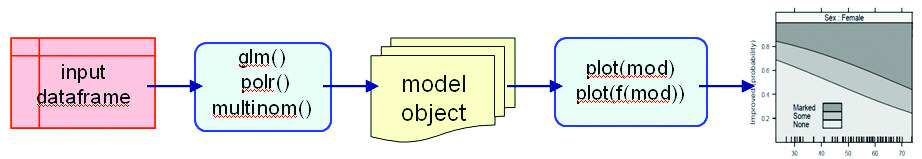
\includegraphics[width=\textwidth]{fig/goverview-R1}
  \end{center}
\end{frame}

\section{Proportional odds model}
\begin{frame}[fragile]
  \frametitle{Ordinal response: Proportional odds model}
Arthritis treatment data:
\begin{Output}[baselinestretch=.8]
                          Improvement
  Sex   Treatment    None    Some   Marked    Total
  ---   ---------    ---------------------    -----
   F     Active        6       5      16        27
   F     Placebo      19       7       6        32

   M     Active        7       2       5        14
   M     Placebo      10       0       1        11
\end{Output}
  \begin{itemize}
	\item Model logits for adjacent category cutpoints:

  \[
  \mbox{logit} \,  ( \theta_{ij1} )
 = \log  \frac{ \pi_{ij1} } { \pi_{ij2}  +  \pi_{ij3} }
 = \mbox{logit ( None vs. [Some or Marked] )}
  \]
  \[
  \mbox{logit} \,  ( \theta_{ij2} )
 = \log  \frac{ \pi_{ij1}  +  \pi_{ij2} } { \pi_{ij3} }
 = \mbox{logit ( [None or Some] vs. Marked)}
  \]
  \end{itemize}
% 
\end{frame}

%\framebreak
\begin{frame}
  \begin{itemize}
	\item Consider a logistic regression model for each logit:
  \begin{equation*} 
  \mbox{logit} ( \theta_{ij1} )
 = \alpha _1  +  \vec{x} '_{ij} \,  \vec{\beta} _1 \quad\quad\mbox{  None vs. Some/Marked}
  \end{equation*}
  \begin{equation*} 
  \mbox{logit} ( \theta_{ij2} )
 = \alpha _2  +  \vec{x} '_{ij} \,  \vec{\beta} _2 \quad\quad\mbox{  None/Some vs. Marked}
  \end{equation*}

	\item Proportional odds assumption: 
	\alert{regression functions are parallel} on the logit scale
	i.e., \(\vec{\beta}_1 = \vec{\beta} _2\).

\begin{center}
  \includegraphics[height=.6\textheight]{fig/podds}
\end{center}
  \end{itemize}
\end{frame}


\subsection{Latent variable interpretation}
\begin{frame}
 \frametitle{Proportional odds: Latent variable interpretation}
A simple motivation for the proportional odds model:
\begin{itemize}
 \item Imagine a continuous, but \emph{unobserved} response, $\xi$,
  a linear function of predictors
\begin{equation*}
\xi_i = \vec{\beta}\trans \vec{x}_i + \epsilon_i
\end{equation*}

 \item The \emph{observed} response, Y, is discrete, according to
 some \emph{unknown} thresholds,
 $\alpha_1 < \alpha_2, <\cdots < \alpha_{m-1}$
 \item That is, the response, $Y = i$ if $ \alpha_i \le \xi_i < \alpha_{i+1}$
 \item Thus, intercepts in the proportional odds model $\sim$ 
thresholds on $\xi$
\end{itemize}

\begin{center}
 \includegraphics[width=.8\textwidth]{fig/prop-odds1}
\end{center}
\end{frame}

\begin{frame}
 \frametitle{Proportional odds: Latent variable interpretation}
We can visualize the relation of the latent variable $\xi$ to
the observed response $Y$, for two values, $x_1$ and $x_2$,
of a single predictor, $X$ as shown below:
\begin{center}
 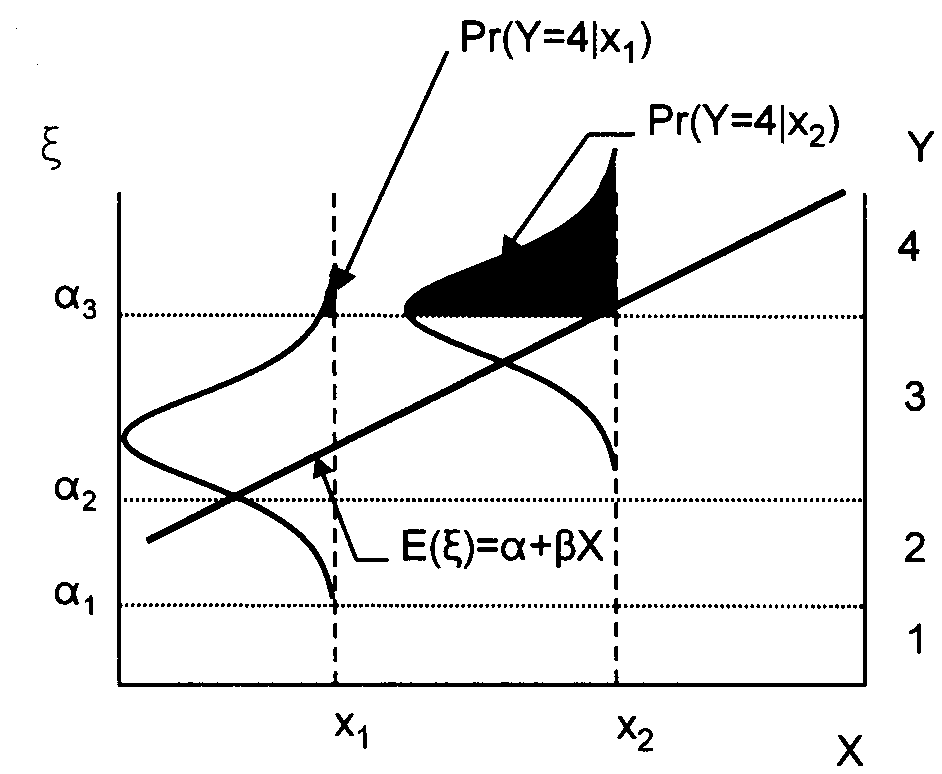
\includegraphics[width=.6\textwidth]{fig/prop-odds2}
\end{center}
\end{frame}

\begin{frame}
 \frametitle{Proportional odds: Latent variable interpretation}
For the Arthritis data, the relation of improvement to age is
shown below (using the R \pkg{effects})
\begin{center}
 \includegraphics[width=.9\textwidth]{fig/arthritis-propodds4}
\end{center}
\end{frame}


\subsection{Fitting and plotting in SAS}
\begin{frame}[fragile]
  \frametitle{Proportional odds model: Fitting and plotting}
Similar to binary response models, except:
  \begin{itemize*}
	\item Response variable has $m>2$ levels;  \ODS\ has \verb|_LEVEL_| variable
	\item Must ensure that response levels are ordered as you want---
	use \texttt{order=data} or \texttt{descending} options.
	\item Validity of analysis depends on proportional odds assumption.
	Test of this assumption appears in \PROC{LOGISTIC} output.
  \end{itemize*}
Example, using dependent variable \texttt{improve}, with values 0, 1, and 2:
\vspace{1ex}
\begin{Input}[fontsize=\small,label=\fbox{\texttt{glogist2a.sas} $\cdots$},baselinestretch=0.8]
proc logistic data=arthrit \sasemph{descending};
   class sex (ref=last) treat (ref=first) / param=ref;
   model  \sasemph{improve} = sex  treat  age ;
   output out=results p=prob l=lower u=upper
          xbeta=logit stdxbeta=selogit / alpha=.33;

proc print data=results(obs=6);
   id id treat sex;
   var improve _level_ prob lower upper logit;
   format prob lower upper logit selogit 6.3;
run;
\end{Input}
\end{frame}
%\framebreak

\begin{frame}[fragile]
The response profile displays the ordering of the outcome variable (\alert{decreasing} here)
\begin{Output}[gobble=6,fontsize=\footnotesize,baselinestretch=0.8]
                                Response Profile
 
                       Ordered                      Total
                         Value      improve     Frequency

                             1            2            28
                             2            1            14
                             3            0            42
\end{Output}
Test of Proportional Odds Assumption: OK
\begin{Output}[gobble=6,fontsize=\footnotesize,baselinestretch=0.8]
                 Score Test for the Proportional Odds Assumption
 
                       Chi-Square       DF     Pr > ChiSq
                           \sasemph{2.4916        3         0.4768}
\end{Output}
Parameter estimates ($\beta_i$):
\begin{Output}[gobble=2,fontsize=\footnotesize,baselinestretch=0.8]
                   Analysis of Maximum Likelihood Estimates
 
                                      Standard        Wald
  Parameter           DF   Estimate      Error    Chi-Square  Pr > ChiSq

  Intercept 2          1    -4.6826     1.1949      15.3566      <.0001
  Intercept 1          1    -3.7836     1.1530      10.7680      0.0010
  sex       Female     1     1.2515     0.5321       5.5330      0.0187
  treat     Treated    1     1.7453     0.4772      13.3774      0.0003
  age                  1     0.0382     0.0185       4.2361      0.0396
\end{Output}
\end{frame}

\begin{frame}[fragile]
Odds ratios ($\exp(\beta_i)$)
\begin{Output}[gobble=5,fontsize=\footnotesize,baselinestretch=0.9]
                              Odds Ratio Estimates
                                        
                                         Point          95% Wald
          Effect                      Estimate      Confidence Limits

          sex   Female vs Male           3.496       1.232       9.918
          treat Treated vs Placebo       5.728       2.248      14.594
          age                            1.039       1.002       1.077
\end{Output}
i.e., Treated 5.73 times as likely to show more improvement.
\vspace{1.5ex}

Output data set (\texttt{RESULTS}) for plotting:
\begin{Output}[gobble=2,fontsize=\footnotesize,baselinestretch=0.9]
  id    treat    sex  improve  _LEVEL_   prob   lower   upper   logit

  57   Treated   Male     1       2      0.129   0.069   0.229  -1.907
  57   Treated   Male     1       1      0.267   0.157   0.417  -1.008
   9   Placebo   Male     0       2      0.037   0.019   0.069  -3.271
   9   Placebo   Male     0       1      0.085   0.048   0.149  -2.372
  46   Treated   Male     0       2      0.138   0.076   0.238  -1.830
  46   Treated   Male     0       1      0.283   0.171   0.429  -0.931
  ...
\end{Output}
\end{frame}

\begin{frame}[fragile]
To plot predicted probabilities in a single graph, combine values of \texttt{TREAT} and
\verb|_LEVEL_|
\begin{Input}[fontsize=\small,label=\fbox{$\cdots$ \texttt{glogist2a.sas} $\cdots$},baselinestretch=0.8,firstnumber=13]
   \sascomment{*-- combine treatment and _level_, set error bar color;}
data results;
   set results;
   treatl = trim(treat)||put(_level_,1.0); 
   if treat='Placebo' then col='BLACK';
                      else col='RED';
proc sort data=results;
   by sex treatl age;
\end{Input}
$\cdots$ \texttt{plot prob * age = treatl; by sex;}
\begin{center}
 \begin{minipage}[b]{.35\linewidth}
  \centering
  \includegraphics[width=.99\linewidth]{fig/glogist2a1}
 \end{minipage}%
 \begin{minipage}[b]{.35\linewidth}
  \centering
  \includegraphics[width=.99\linewidth]{fig/glogist2a2}
 \end{minipage}
\end{center}
\end{frame}

%\framebreak
\begin{frame}[fragile]
Add error bars and legends:
\vspace{2ex}
\begin{Input}[fontsize=\small,label=\fbox{$\cdots$ \texttt{glogist2a.sas} $\cdots$},baselinestretch=0.8,firstnumber=22]
   \sascomment{*-- Error bars, on prob scale;}
%bars(data=results, var=prob, 
   class=age, cvar=treatl, by=age,
   lower=lower, upper=upper, 
   color=col, out=bars);
proc sort data=bars;
   by sex treatl age;

   \sascomment{*-- Custom legends, for treat-level and sex;}
%label(data=results, y=prob, x=age, xoff=1, cvar=treatl,
   by=sex, subset=last.treatl, out=label1, pos=6, text=treatl);
%label(data=results, y=0.9, x=20, size=2,
   by=sex, subset=first.sex, out=label2, pos=6, text=sex);

   \sascomment{*-- Combine the annotate data sets;}
data \sasemph{bars};
   set label1 label2 bars;
   by sex;
\end{Input}
\end{frame}

%\framebreak
\begin{frame}[fragile]
Plot step:
\begin{Input}[fontsize=\small,label=\fbox{$\cdots$ \texttt{glogist2a.sas}},baselinestretch=0.8,firstnumber=41]
goptions hby=0;
proc gplot data=results;
   plot \sasemph{prob * age = treatl} / 
       vaxis=axis1 haxis=axis2 hminor=1 vminor=1
       nolegend \sasemph{anno=bars} name=glogist2a';
   \sasemph{by sex;}
   axis1 label=(a=90 'Prob. Improvement (67% CI)')
         order=(0 to 1 by .2);
   axis2 order=(20 to 80 by 10)
         offset=(2,5);
   symbol1 v=circle  i=join line=3 c=black;
   symbol2 v=circle  i=join line=3 c=black;
   symbol3 v=dot     i=join line=1 c=red;
   symbol4 v=dot     i=join line=1 c=red;
run;
\end{Input}
\end{frame}

\begin{frame}
% two figures 
 \begin{minipage}[b]{.5\linewidth}
  \centering
  \includegraphics[width=.99\linewidth]{fig/glogist2a1}
 \end{minipage}%
 \begin{minipage}[b]{.5\linewidth}
  \centering
  \includegraphics[width=.99\linewidth]{fig/glogist2a2}
 \end{minipage}
\begin{itemize*}
  \item Intercept1: Marked , Some | None
  \item Intercept2: Marked | Some, None
  \item On logit scale, these would be parallel lines
  \item Effects of age, treatment, sex similar to what we saw before
\end{itemize*}
\end{frame}

\begin{frame}[fragile]
 \frametitle{Effect plots using SAS ODS}
\begin{Input}[fontsize=\footnotesize,label=\fbox{\texttt{arthritis-propodds-ods.sas}},baselinestretch=0.8]
ods graphics on ;
proc logistic data=arthrit descending  ;
   class sex (ref=last) treat (ref=first) / param=ref;
   model  improve = sex  treat  age / clodds=wald expb;
   \sasemph{effectplot slicefit}(sliceby=improve plotby=Treat) / at(sex=all) clm alpha=0.33;
   \sasemph{effectplot interaction}(sliceby=improve x=Treat) / at(sex=all) clm alpha=0.33;
run;
ods graphics off;
\end{Input}
\begin{center}
 \begin{minipage}[b]{.5\linewidth}
  \centering
  \includegraphics[width=.99\linewidth]{fig/arthritis-propodds-ods1}
 \end{minipage}%
% \hspace{2mm}
 \begin{minipage}[b]{.5\linewidth}
  \centering
  \includegraphics[width=.99\linewidth]{fig/arthritis-propodds-ods2}
 \end{minipage}
\end{center}
\end{frame}

\subsection{Proportional odds models in R}
\begin{frame}[fragile]
   \frametitle{Proportional odds models in R}
  \begin{itemize}
	\item{\bfseries Fitting: \func{polr}} in \pkg{MASS}
%	\item{\large\bfseries Plotting:}
  \end{itemize}
The response, \texttt{Improved} has been defined as an \emph{ordered} factor
\begin{Rin}
> factor(Arthritis$Improved)
\end{Rin}
\begin{Rout}[fontsize=\footnotesize]
 [1] Some   None   None   Marked Marked Marked None   Marked  None
 ...
[81] None   Some   Some   Marked
\sasemph{Levels: None < Some < Marked}
\end{Rout}
% \KileResetHL \KateResetHL
Fitting:
\begin{Rin}
library(vcd)
library(car)         # for Anova()

arth.polr <- polr(Improved ~ Sex + Treatment + Age, 
                  data=Arthritis)
summary(arth.polr)
Anova(arth.polr)      # Type II tests
\end{Rin}

\end{frame}

\begin{frame}[fragile,plain]
%    \frametitle{Proportional odds models in R}
%   \begin{itemize}
% 	\item{\large\bfseries Fitting: \func{polr}} in \pkg{MASS}
% %	\item{\large\bfseries Plotting:}
%   \end{itemize}
The \func{summary} function gives standard statistical results:
\begin{Rin}
> summary(arth.polr)
\end{Rin}
%Output:
\begin{Rout}[baselinestretch=0.8,fontsize=\footnotesize]
Call:
polr(formula = Improved ~ Sex + Treatment + Age, data = Arthritis)

Coefficients:
                       Value Std. Error   t value
SexMale          -1.25167969 0.54636501 -2.290922
TreatmentTreated  1.74528949 0.47589542  3.667380
Age               0.03816199 0.01841628  2.072187

Intercepts:
            Value   Std. Error t value
None|Some    2.5319  1.0571     2.3952
Some|Marked  3.4309  1.0912     3.1442

Residual Deviance: 145.4579 
AIC: 155.4579
\end{Rout} 
\begin{Rin}
> Anova(arth.polr)      # Type II tests
\end{Rin}
%Output:
\begin{Rout}[baselinestretch=0.8,fontsize=\footnotesize]
Anova Table (Type II tests)

Response: Improved
          LR Chisq Df Pr(>Chisq)    
Sex         5.6880  1  0.0170812 *  
Treatment  14.7095  1  0.0001254 ***
Age         4.5715  1  0.0325081 *  
---
Signif. codes:  0 '***' 0.001 '**' 0.01 '*' 0.05 '.' 0.1 ' ' 1  
\end{Rout} 

\end{frame}

\begin{frame}[fragile]
   \frametitle{Proportional odds models in R: Plotting}
  \begin{itemize}
%	\item{\large\bfseries Fitting}: \func{polr} in \pkg{MASS}
	\item{\bfseries Plotting: \code{plot(effect())}}  in \pkg{effects}
  \end{itemize}
\begin{Rin}[baselinestretch=0.8]
> library(effects)
> plot(effect("Treatment:Age", arth.polr))
\end{Rin}
\begin{minipage}[c]{.49\linewidth}
 \centering
 \includegraphics[width=\linewidth]{fig/arthritis-propodds}
\end{minipage}
\begin{minipage}[c]{.49\linewidth}
  \begin{itemize}
   \item The default plot shows all details
   \item But, is harder to compare across treatment and response levels
  \end{itemize}


\end{minipage}

% \begin{center}
%  \includegraphics[height=.65\dispheight]{fig/arthritis-propodds}
% \end{center}

\end{frame}

\begin{frame}[fragile]
   \frametitle{Proportional odds models in R: Plotting}
%   \begin{itemize}
% %	\item{\large\bfseries Fitting}: \func{polr} in \pkg{MASS}
% 	\item{\bfseries Plotting: \code{plot(effect())}}  in \pkg{effects}
%   \end{itemize}
Making visual comparisons easier:
\begin{Rin}[baselinestretch=0.8]
> plot(effect("Treatment:Age", arth.polr), style='stacked')
\end{Rin}
\begin{center}
 \includegraphics[height=.7\dispheight]{fig/arthritis-propodds2}
\end{center}

\end{frame}

\begin{frame}[fragile]
   \frametitle{Proportional odds models in R: Plotting}
%   \begin{itemize}
% %	\item{\large\bfseries Fitting}: \func{polr} in \pkg{MASS}
% 	\item{\bfseries Plotting: \code{plot(effect())}}  in \pkg{effects}
%   \end{itemize}
Making visual comparisons easier:
\begin{Rin}[baselinestretch=0.8]
> plot(effect("Sex:Age", arth.polr), style='stacked')
\end{Rin}
\begin{center}
 \includegraphics[height=.7\dispheight]{fig/arthritis-propodds3}
\end{center}

\end{frame}

\begin{frame}[fragile]
   \frametitle{Proportional odds models in R: Plotting}
These plots are even simpler on the logit scale, using \texttt{latent=TRUE} to show the
cutpoints between response categories
\begin{Rin}
> plot(effect("Treatment:Age", arth.polr, latent=TRUE))
\end{Rin}
\begin{center}
 \includegraphics[height=.7\dispheight]{fig/arthritis-propodds5}
\end{center}

\end{frame}



\endinput

% slide template
\begin{frame}
  \frametitle{}
  \begin{itemize}
	\item{\large\bfseries }
      \begin{itemize*}
	  \item 
    	\begin{itemize*}
		\item 
		\item 
		\end{itemize*}
	  \item 
	  \end{itemize*}
	\item{\large\bfseries }
	\item{\large\bfseries }
  \end{itemize}
\end{frame}

